\documentclass[a4paper]{article}

\usepackage{fullpage} % Package to use full page
\usepackage{parskip} % Package to tweak paragraph skipping
\usepackage{tikz} % Package for drawing
\usepackage{amsmath}
\usepackage{hyperref}
\usepackage{listings} % iPackage for code
\usepackage{amsthm}
\usepackage{amsmath}
\usepackage{amssymb}
\usepackage{bbm}

\title{CSC411 Fall 2017\\Assignment 3 Report}
\author{Tianbao Li}
\date{2017/12/04}

\begin{document}

\maketitle

\section{20 Newsgroups prediction}

\subsection{Data summary}

Here is the detailed information of the dataset:

\begin{itemize}
    \item data set: \href{http://scikit-learn.org/stable/datasets/twenty_newsgroups.html}{The 20 newsgroups text}
    \item data amount: 11314
    \item feature amount: 101631
    \item data representation: tf-idf
    \item baseline: Bernoulli Naive-Bayes classifier
\end{itemize}

\subsection{Model training}

To train model to outperform the baseline, here we useopen-souece code of \href{http://scikit-learn.org/stable/}{scikit-learn}. Here, I picked several different algorithms and trained their hyper-parameters with k-fold validation. The detailed better hyper-parameters, train losses (0-1 loss), test losses (0-1 loss) are shown in Table~\ref{tab: Model_comparison}. From the result of the validation losses, the best three models are Neural Networks, Multinomial Naive Bayes, Logist Regression, and has the same best results in test dataset.

\begin{table}[htbp]
\centering
\begin{tabular}{|c|c|c|c|}
    \hline
    Model & Hyper-pramater & Train loss & test loss\\
    \hline
    BernoulliNB &  & 0.598727240587 & 0.457912904939\\
    \hline
    MultinomialNB & $\alpha=0.01$ & 0.958900477285 & 0.700212426978\\
    \hline
    Logist Regression & $C=500$ & 0.974721583878 & 0.683483802443\\
    \hline
    SGD & $\alpha=0.0001$ & 0.962877850451 & 0.671136484334\\
    \hline
    SVM & $C=1$ & 0.895704436981 & 0.67750929368\\
    \hline
    KNN & $K=1$ & 0.973749337104 & 0.113382899628\\
    \hline
    Decision Tree & $K=601$ & 0.974721583878 & 0.4026818906\\
    \hline
    Neural Networks & $\alpha=0.0001$ & 0.947587060279 & 0.712294211365\\
    \hline
    \end{tabular}
\caption{Model comparison}
\label{tab: Model_comparison}
\end{table}

\subsection{Hyper-parameters training}

To train models by choosing better-fitting parameters, I splited training data by \href{http://scikit-learn.org/stable/modules/generated/sklearn.model_selection.KFold.html}{KFold} and run cross valiadation by \href{http://scikit-learn.org/stable/modules/generated/sklearn.model_selection.cross_val_score.html}{cross\_val\_score}.

Here, taking multinomial Naive Bayes as an example. Hyper-parameter $\alpha$ is used for smoothing. I picked several possible $\alpha$ value and compared by validation loss, then chose a better $\alpha$.

\begin{lstlisting}[language = Python]
splits = 5
kf = KFold(splits, shuffle = True, random_state = 0)
As = [1e-10, 1e-8, 1e-6, 1e-4, 1e-2, 0.1, 0.5, 1.0, 2, 5, 10]
scores = []
for a in As:
    model = MultinomialNB(alpha = a)
    score = cross_val_score(model, tfidf_train, train_labels, cv = kf)
    scores.append(np.mean(score))
opt_A_index = int(np.argmax(scores))
opt_A = As[opt_A_index]
\end{lstlisting}

\subsection{Model selection}

For the three well-working models, they have their advantages for solving this problem.

\begin{itemize}
    \item \textbf{Neural Networks} can work well for complex models, especially when it comes deeper.
    \item \textbf{Multinomial Naive Bayes} implements the naive Bayes algorithm for multinomially distributed data, text classification usually holds such structure.
    \item \textbf{Logistic Regression} is famous for linear classification, which the newsgroup data has similar distribution.
\end{itemize}

\subsection{Class confusion}

For the best classifier, Neural Networks, the confusion matrix among 20 groups is shown in Table~\ref{tab: Confusion_matrix}. The two classed that Neural Networks classifier confuses about are class 16 and 18.

\begin{table}[htbp]
\centering
\setlength{\tabcolsep}{2pt}
\begin{tabular}{|cccccccccccccccccccc|}
    \hline
    163 & 6 & 5 & 1 & 1 & 0 & 0 & 4 & 4 & 7 & 5 & 3 & 2 & 11 & 7 & 20 & 7 & 28 & 20 & 38\\
    \hline
    1 & 287 & 26 & 15 & 6 & 49 & 2 & 1 & 1 & 2 & 2 & 8 & 11 & 8 & 11 & 3 & 1 & 1 & 1 & 4\\
    \hline
    3 & 19 & 241 & 37 & 10 & 31 & 2 & 2 & 1 & 0 & 0 & 5 & 15 & 1 & 2 & 1 & 2 & 0 & 0 & 2\\
    \hline
    1 & 9 & 39 & 256 & 22 & 7 & 18 & 1 & 1 & 0 & 0 & 2 & 26 & 1 & 0 & 0 & 1 & 2 & 0 & 2\\
    \hline
    1 & 9 & 12 & 32 & 284 & 5 & 14 & 1 & 1 & 0 & 0 & 2 & 11 & 2 & 1 & 0 & 2 & 0 & 0 & 0\\
    \hline
    0 & 16 & 12 & 4 & 3 & 278 & 0 & 0 & 0 & 0 & 0 & 1 & 2 & 0 & 0 & 0 & 0 & 0 & 1 & 0\\
    \hline
    0 & 4 & 3 & 10 & 8 & 4 & 305 & 10 & 5 & 3 & 0 & 1 & 10 & 3 & 3 & 0 & 1 & 0 & 0 & 1\\
    \hline
    15 & 7 & 17 & 9 & 21 & 5 & 20 & 322 & 32 & 15 & 12 & 19 & 21 & 22 & 23 & 14 & 19 & 8 & 13 & 10\\
    \hline
    3 & 5 & 4 & 0 & 4 & 1 & 6 & 16 & 312 & 3 & 1 & 2 & 10 & 7 & 5 & 1 & 4 & 7 & 1 & 2\\
    \hline
    4 & 2 & 1 & 0 & 1 & 2 & 3 & 3 & 3 & 334 & 11 & 8 & 2 & 0 & 1 & 3 & 2 & 3 & 0 & 1\\
    \hline
    2 & 0 & 0 & 1 & 0 & 0 & 0 & 1 & 0 & 14 & 354 & 0 & 0 & 4 & 1 & 0 & 0 & 1 & 2 & 0\\
    \hline
    2 & 6 & 6 & 2 & 2 & 4 & 1 & 2 & 1 & 1 & 0 & 289 & 13 & 0 & 0 & 0 & 7 & 3 & 1 & 1\\
    \hline
    4 & 9 & 2 & 24 & 21 & 5 & 8 & 15 & 18 & 3 & 1 & 14 & 245 & 10 & 9 & 1 & 2 & 1 & 3 & 1\\
    \hline
    2 & 0 & 2 & 0 & 0 & 0 & 0 & 1 & 3 & 3 & 1 & 2 & 8 & 300 & 5 & 2 & 2 & 2 & 5 & 6\\
    \hline
    9 & 7 & 11 & 1 & 1 & 3 & 3 & 3 & 6 & 1 & 1 & 3 & 9 & 3 & 302 & 4 & 7 & 0 & 8 & 6\\
    \hline
    53 & 1 & 3 & 0 & 0 & 1 & 1 & 1 & 2 & 4 & 4 & 3 & 2 & 7 & 6 & 321 & 9 & 13 & 5 & 68\\
    \hline
    9 & 1 & 2 & 0 & 1 & 0 & 3 & 2 & 3 & 2 & 2 & 19 & 1 & 5 & 4 & 0 & 258 & 6 & 89 & 20\\
    \hline
    9 & 1 & 2 & 0 & 0 & 0 & 1 & 2 & 0 & 1 & 2 & 3 & 3 & 3 & 1 & 0 & 8 & 287 & 6 & 6\\
    \hline
    7 & 0 & 4 & 0 & 0 & 0 & 2 & 5 & 4 & 4 & 2 & 10 & 2 & 8 & 13 & 5 & 18 & 13 & 149 & 11\\
    \hline
    31 & 0 & 2 & 0 & 0 & 0 & 1 & 4 & 1 & 0 & 1 & 2 & 0 & 1 & 0 & 23 & 14 & 1 & 6 & 72\\
    \hline
    \end{tabular}
\caption{Confusion matrix}
\label{tab: Confusion_matrix}
\end{table}

\section{Training SVM with SGD}

\subsection{SGD with momentum}

Parameters:
\begin{itemize}
    \item function: $f(w)=0.01w^2$
    \item initianlization: $w_0=10.0$
    \item learning rate: $\alpha=1.0$
    \item momentum: $\beta_1=0.0, \beta_2=0.9$
\end{itemize}

Changes for $w_t$ is shown as Figure~\ref{fig: SGD}.

\begin{figure}[htbp]
\centering
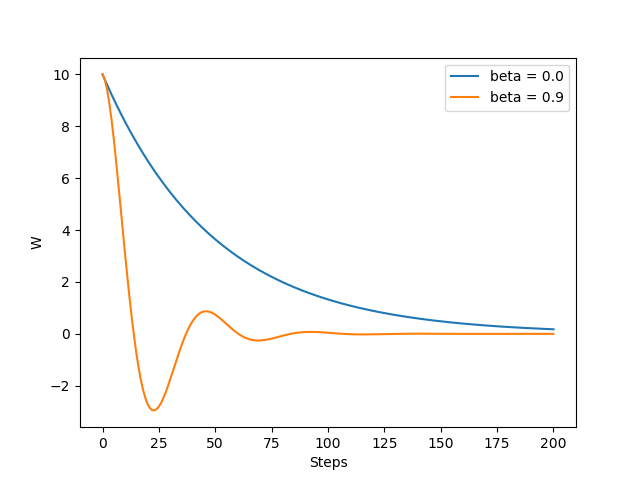
\includegraphics[width = 8cm]{SGD}
\caption{$w_t$ for $\beta=0.0$ and $0.9$}
\label{fig: SGD}
\end{figure}

\subsection{Training SVM}

Given the formula of SVM, the gradient during training can be shown as

\begin{equation}
\frac{\partial \ell}{\partial w}=\left\{
\begin{aligned}
-C*y^{(i)}\mathbf{x}^{(i)}+w & = & y^{(i)}(w^{\mathrm{T}}\mathbf{x}^{(i)}+b)<1 \\
0 & = & y^{(i)}(w^{\mathrm{T}}\mathbf{x}^{(i)}+b)\ge1
\end{aligned}
\right.
\end{equation}

\subsection{Apply on 4-vs-9 digits on MNIST}

Here, I trained SVM on MNIST. The trained models for $\beta=0$ is reported as follows:

\begin{itemize}
    \item $\beta$: 0.0
    \item optimal hyper-parameter: $C=1$
    \item training loss: 0.748119588312
    \item test loss: 0.720131532536
    \item training accuracy: 0.927437641723
    \item test accuracy: 0.92636924193
\end{itemize}

The trained models for $\beta=0.0$ is reported as follows:

\begin{itemize}
    \item $\beta$: 0.1
    \item optimal hyper-parameter: $C=1$
    \item training loss: 0.483890097883
    \item test loss: 0.500220862748
    \item training accuracy: 0.940770975057
    \item test accuracy: 0.937250634748
\end{itemize}

The $w$ figures for $\beta=0.0$ and $0.1$ are shown in Figure ~\ref{fig: SVM}.

\begin{figure}[htbp]
\centering
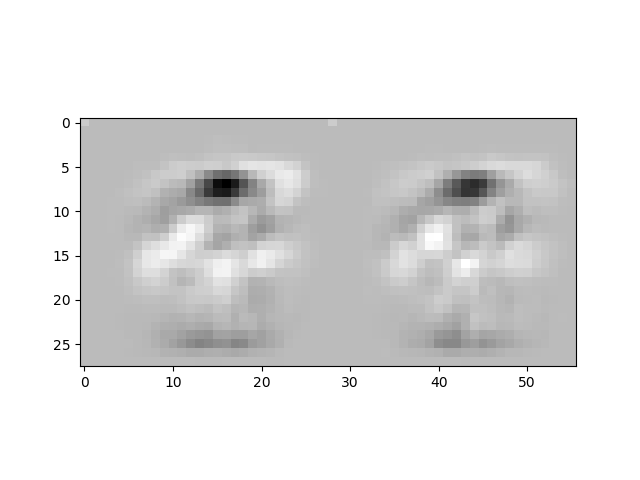
\includegraphics[width = 8cm]{SVM}
\caption{$w$ figure for $\beta=0.0$ (left) and $0.1$ (right)}
\label{fig: SVM}
\end{figure}

\section{Kernels}

\subsection{Positive semidefinite and quadratic form}

Proof that a symmetric matrix $K\in\mathbbm{R}^{d\times d}$ is positive semidefinite iff for all vectors $\mathbf{x}\in\mathbbm{R}^d$ we have $\mathbf{x}^\mathrm{T}K\mathbf{x}\ge0$.

\begin{proof}
    Necessity:
    \begin{align*}
        \because&\forall \mathbf{x}\in\mathbbm{R}^d, \mathbf{x}^\mathrm{T}K\mathbf{x}\ge0\\
        \therefore&\forall v \text{ as eigenvector of } K, v^\mathrm{T}Kv=v^\mathrm{T}\lambda v\ge0\\
        \therefore&\lambda\ge0\text{ ($\lambda$ corresponds to $v$)}\\
        \therefore&\forall\lambda\ge0\text{ as eigenvalue of } K\\
        \therefore&K\text{ has no negative eigenvalue}\\
        \because&K\text{ is symmetric}\\
        \therefore&K\text{ is positive semidefinite}
    \end{align*}
    \quad\quad\quad Sufficiency:
    \begin{align*}
        \because&K\in\mathbbm{R}^{d\times d}\text{ is symmetric}\\
        \therefore&K\text{ has orthogonal eigenvectors for different eigenvalues}\\
        &K\text{ can be diagonalized}\\
        \therefore&K\text{ can be represented as }K=Q\Lambda Q^{-1}=Q\Lambda Q^\mathrm{T}\\
        &Q=[v_1,v_2,\dots,v_d]^\mathrm{T}:\text{ eigenvector matrix}\\
        &\Lambda:\text{ diagonal matrix}\\
        \because&v_1,v_2,\dots,v_d\text{ are diagonal}\\
        \therefore&\forall\mathbf{x}\in R^d=(c_1v_1+c_2c_2+\dots+c_dv_d)\\
        \therefore&\mathbf{x}^\mathrm{T}A\mathbf{x}=\mathbf{x}^\mathrm{T}Q\Lambda Q^\mathrm{T}\mathbf{x}\\
        &\quad\quad=(c_1v_1+c_2c_2+\dots+c_dv_d)\bigl(\begin{smallmatrix} v_1\\v_2\\\vdots\\v_d\end{smallmatrix}\bigr)\bigl(\begin{smallmatrix} \lambda_1 &  &  &\\\  & \lambda_2 &  &\\  &  & \dots &\\  &  &  & \lambda_d\\\end{smallmatrix}\bigr)(v_1,v_2,\dots,v_d)(c_1v_1+c_2c_2+\dots+c_dv_d)^\mathrm{T}\\
        &\quad\quad=(c_1||v_1||^2+c_2||v_2||^2+\dots+(c_d||v_d||^2))\bigl(\begin{smallmatrix} \lambda_1 &  &  &\\\  & \lambda_2 &  &\\  &  & \dots &\\  &  &  & \lambda_d\\\end{smallmatrix}\bigr)(c_1||v_1||^2+c_2||v_2||^2+\dots+(c_d||v_d||^2))^\mathrm{T}\\
        &\quad\quad=\lambda_1c_1^2||v_1||^4+\lambda_2c_2^2||v_2||^4+\dots+\lambda_dc_d^2||v_d||^4\ge0\\
        \therefore&\mathbf{x}^\mathrm{T}K\mathbf{x}\ge0
    \end{align*}
\end{proof}


\bibliographystyle{plain}
\bibliography{bibliography.bib}
\end{document}


Given:

\begin{equation}
    p(y=k)=a_k
\end{equation}

\begin{equation}
    p(\mathbf{x}|y=k,\mu,\sigma)=(\prod^d_{i=1}2\pi\sigma^2_i)^{-1/2}\exp\{-\sum^d_{i=1}\frac{1}{2\sigma^2_i}(x_i-\mu_{ki})^2\}
\end{equation}

\subsection{Bayes' rule derivation}

\begin{align*}
    p(y=k|\mathbf{x},\mu,\sigma)&=\frac{p(\mathbf{x}|y=k,\mu,\sigma)p(y=k)}{p(\mathbf{x}|\mu,\sigma)}\\
    &=\frac{p(\mathbf{x}|y=k,\mu,\sigma)p(y=k)}{\sum^K_{j=1}p(\mathbf{x}|y=j,\mu,\sigma)}\\
    &=\frac{(\prod^d_{i=1}2\pi\sigma^2_i)^{-1/2}\exp\{-\sum^d_{i=1}\frac{1}{2\sigma^2_i}(x_i-\mu_{ki})^2\}a_k}{\sum^K_{j=1}(\prod^d_{i=1}2\pi\sigma^2_i)^{-1/2}\exp\{-\sum^d_{i=1}\frac{1}{2\sigma^2_i}(x_i-\mu_{ji})^2\}}
\end{align*}

\subsection{Negative likelihood function (NLL)}

\begin{align*}
    \ell(\theta;D)&=-\log p(y^{(1)},\mathbf{x}^{(1)},y^{(2)},\mathbf{x}^{(2)},\dots,y^{(N)},\mathbf{x}^{(N)}|\theta)\\
    &=-\log\prod^N_{n=1}p(y^{(n)},x^{(n)}|\theta)\\
    &=-\sum^N_{n=1}(\log p(x^{(n)}|y^{(n)},
    \theta)+\log p(y^{(n)}|\theta))\\
    &=-\sum^N_{n=1}(\log((\prod^d_{i=1}2\pi\sigma^2_i)^{-1/2}\exp\{-\sum^d_{i=1}\frac{1}{2\sigma^2_i}(x_i^{(n)}-\mu_{ki})^2\})+\log\alpha_k)\\
    &=-\sum^N_{n=1}(-\frac{1}{2}\sum^d_{i=1}\log(2\pi\sigma^2_i)-\sum^d_{i=1}\frac{1}{2\sigma^2_i}(x^{(n)}_i-\mu_{ki})^2+\log\alpha_k)\\
    &=\sum^N_{n=1}(\sum^d_{i=1}\log(\pi\sigma^2_i)+\sum^d_{i=1}\frac{1}{2\sigma^2_i}(x^{(n)}_i-\mu_{ki})^2-\log\alpha_k)
\end{align*}

\subsection{Partial derivatives}

\begin{align*}
    \frac{\partial \ell}{\partial \mu_{ki}}&=\frac{\partial(\sum^N_{n=1}\sum^d_{i=1}\frac{1}{2\sigma^2_i}(x^{(n)}_i-\mu_{ki})^2)}{\partial \mu_{ki}}\\
    &=-\sum^N_{n=1}\sum^d_{i=1}\frac{1}{\sigma^2_i}\mathbbm{1}(y^{(n)}=k)(x^{(n)}_i-\mu_{ki})\\
    \frac{\partial \ell}{\partial \sigma_i^2}&=\frac{\partial(\sum^N_{n=1}(\sum^d_{i=1}\log(\pi\sigma^2_i)+\sum^d_{i=1}\frac{1}{2\sigma^2_i}(x^{(n)}_i-\mu_{ki})^2))}{\partial \sigma_i^2}\\
    &=\sum^N_{n=1}\sum^d_{i=1}\mathbbm{1}(y^{(n)}=k)(\frac{1}{\sigma^2_i}-\frac{1}{2\sigma^4_i}(x^{(n)}_i-\mu_{ki})^2)
\end{align*}

\subsection{Estimation}

\begin{align*}
    \frac{\partial \ell}{\partial \mu_{ki}}&=0\\
    \Rightarrow\mu_{ki}&=\frac{\sum^N_{n=1}\sum^d_{i=1}\mathbbm{1}(y^{(n)}=k)x^{(n)}_i}{\sum^N_{n=1}\sum^d_{i=1}\mathbbm{1}(y^{(n)}=k)}\\
    \frac{\partial \ell}{\partial \sigma_i^2}&=0\\
    \Rightarrow\sigma_i&=\sqrt{\frac{\sum^N_{n=1}\sum^d_{i=1}\mathbbm{1}(y^{(n)}=k)*(x^{(n)}_i-\mu_{ki})^2}{2\sum^N_{n=1}\sum^d_{i=1}\mathbbm{1}(y^{(n)}=k)}}
\end{align*}

\section{Handwritten digit classification}

In this assignemnt, we use the dataset of handwritten digit. To get a macro view of the data, here we plot the means for each data classes in the training set, shown in Figure~\ref{fig: Trainging_data_mean}.

\begin{figure}[htbp]
\centering
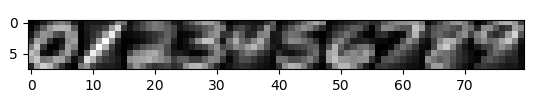
\includegraphics[width = 8cm]{Trainging_data_mean}
\caption{Mean for each class}
\label{fig: Trainging_data_mean}
\end{figure}

\subsection{K-NN classifier}

Fisrt, we build a K nearest neighbor classifier using Euclidean distance on the data.

\subsubsection{Accuracy for certain K values}

\begin{itemize}
    \item for K = 1
    \begin{itemize}
        \item train classification accuracy: 1.0
        \item test classification accuracy: 0.96875
    \end{itemize}
    \item for K = 15
    \begin{itemize}
        \item train classification accuracy: 0.961
        \item test classification accuracy: 0.959
    \end{itemize}
\end{itemize}

\subsubsection{Ties solution}

During the implementation, one important problem is that ties usually happens and need to be broken. The solution is shown as follows.

\begin{lstlisting}[language = Python]
def query_knn(self, test_point, k):
    digit = None
    dist = self.l2_distance(test_point)
    noTies = False
    while noTies == False:
        mink = np.argpartition(dist, k)[:k]
        counts = np.bincount(self.train_labels[mink].astype(int))
        digit = np.argwhere(counts == np.amax(counts))
        if len(digit) > 1:
            k = k - 1
        else:
            noTies = True
    return digit
\end{lstlisting}

While running KNN, if ties happen (which means two classes has the same maximum count), we try to decrease k by 1 and run the KNN again until no ties. As the class label should focus on one or a few classes, ties are unlikely to happen when $K=1$, so this should be a solution to get an answer without ties.

\subsubsection{Best k}

Here we implement 10 fold cross validation in range 1-15 to find the optimal K. By finding minimun validation error, optimal K for this problem is that $K=3$ and accuracies are shown as follows.

\begin{itemize}
    \item train classification accuracy: 1.0
    \item valiadation classification accuracy: 0.96514286
    \item test classification accuracy: 0.96875
\end{itemize}

\subsection{Conditional gaussian classifier training}

\subsubsection{Diagonal covariance}

The diagonal elements of each covariance matrix $\Sigma_k$ can be plotted as Figure~\ref{fig: Diagomal_covariance}.

\begin{figure}[htbp]
\centering
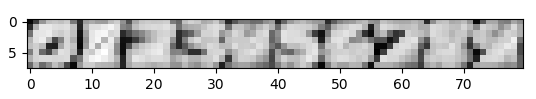
\includegraphics[width = 8cm]{Diagomal_covariance}
\caption{Diagonal elements of covariance for each class}
\label{fig: Diagomal_covariance}
\end{figure}

\subsubsection{Average conditional log-likelihood}

The average conditional log-likelihood for each class is shown as follows.

\begin{itemize}
    \item training data avg conditional likelihood: [-2.78902836 -2.48009327 -2.46864922 -2.53467722\\-2.49894322 -2.93938866
 -2.4646036  -3.70354979 -2.47281232 -2.74221317]
    \item test data avg conditional likelihood: [-3.22599621 -4.13098548 -2.44591828 -3.1675836\\-2.65604537 -3.69867522
 -3.67902811 -7.62636215 -2.81381993 -3.95651773]
\end{itemize}

\subsubsection{Accuracy}

By selecting the most likely posterior class for each datapoint as prediction, the accuracy is shown as follows.

\begin{itemize}
    \item training accuracy: 0.981285714286
    \item test accuracy: 0.9605
\end{itemize}

\subsubsection{Leading eigenvectors}

The leading eigenvectors of each covariance matrix $\Sigma_k$ can be plotted as Figure~\ref{fig: Leading_eigenvectors}.

\begin{figure}[htbp]
\centering
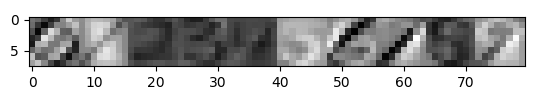
\includegraphics[width = 8cm]{Leading_eigenvectors}
\caption{Leading eigenvectors of covariance for each class}
\label{fig: Leading_eigenvectors}
\end{figure}

\subsection{Naive bayes classifier training}

\subsubsection{Convert to binart features}

\begin{lstlisting}[language = Python]
def binarize_data(pixel_values):
    return np.where(pixel_values > 0.5, 1.0, 0.0)
\end{lstlisting}

\subsubsection{Model fitting}

For a Bernoulli Naive Bayes classifier using MAP, we need to calculate $\eta$ first.

\begin{lstlisting}[language = Python]
def compute_parameters(train_data, train_labels):
    eta = np.zeros((10, 64))
    K = eta.shape[0]
    d = eta.shape[1]
    for k in range(K):
        k_index = np.argwhere(train_labels == k)
        k_digits = train_data[k_index].reshape(-1, d)
        for j in range(d):
            eta[k][j] = (np.sum(k_digits[:, j]) + 1.0)\
                        / (k_digits.shape[0] + 2.0)
    return eta
\end{lstlisting}

\subsubsection{Plot $\eta$}
The parameters $\eta$ is plotted in Figure~\ref{fig: Plot_eta}.

\begin{figure}[htbp]
\centering
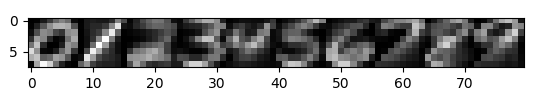
\includegraphics[width = 8cm]{Plot_eta}
\caption{$\eta$ for each class}
\label{fig: Plot_eta}
\end{figure}

\subsubsection{Sample new data}

Given the parameters $\eta$, we can sample new data points for each of the 10 digits. \textit{numpy.random.binomial} method is used here. One new data point is like Figure~\ref{fig: New_data}.

\begin{figure}[htbp]
\centering
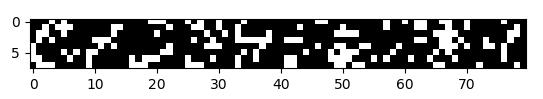
\includegraphics[width = 8cm]{New_data}
\caption{Sampled data point}
\label{fig: New_data}
\end{figure}

\subsubsection{Average conditional log-likelihood}

The average conditional log-likelihood for each class is shown as follows.

\begin{itemize}
    \item training data avg conditional likelihood: [-2.8909254  -3.92355812 -3.26626627 -3.10729808\\-3.01401521 -3.12587265
 -2.94008982 -3.17888068 -3.47393427 -3.54254905]
    \item test data avg conditional likelihood: [-3.10584429 -3.6500495  -3.3475608  -3.29021075\\-3.04145573 -3.20550698
 -3.06688846 -3.23938846 -3.44419131 -3.507459  ]
\end{itemize}

\subsubsection{Accuracy}

By selecting the most likely posterior class for each datapoint as prediction, the accuracy is shown as follows.

\begin{itemize}
    \item training accuracy: 0.774142857143
    \item test accuracy: 0.76425
\end{itemize}

\subsection{Model comparison}

For the handwritten digit classification problem, we use models of KNN, conditional Gaussian and naive Bayes. Analyzing from the accuracy, KNN and conditional Gaussian works better, while Naive Bayes performes badly.

\begin{itemize}
    \item KNN: Due to the relatively distinct classification among digits, decision boundaries are clear in some ways. So it is easy for KNN classifier to find the right group.
    \item conditional Gaussian: Because the pattern for each class seems fixed, so data points for a certain class gather around the mean. Such structure can be easily caught by Gaussian.
    \item naive Bayes: Naive Bayes has the assumption that all features should be i.i.d given a data point. However, as we can see from the figures that each feature corresponds to a pixel in the figure. For a digit, pixel connects with each other and form the shape of the digit. So the features here are not i.i.d. Naive Bayes could not work well upon obeying the assumption.
\end{itemize}
